%!TEX program = xelatex
\documentclass[cs4size,a4paper]{ctexart}   
%==================== 数学符号公式 ============
\usepackage{amsmath}                 % AMS LaTeX宏包
\usepackage[style=1]{mdframed}
\usepackage{amsthm}
\usepackage{amsfonts}

\usepackage{makecell}
\usepackage{mathrsfs}                % 英文花体字 体
\usepackage{bm}                      % 数学公式中的黑斜体
\usepackage{bbding,manfnt}           % 一些图标,如 \dbend
\usepackage{lettrine}                % 首字下沉,命令\lettrine
\def\attention{\lettrine[lines=2,lraise=0,nindent=0em]{\large\textdbend\hspace{1mm}}{}}
\usepackage{longtable}               % 长表格
\usepackage[toc,page]{appendix}
\usepackage{geometry}                % 页边距调整
\geometry{top=3.0cm,bottom=2.7cm,left=2.5cm,right=2.5cm}
%====================公式按章编号==========================
\numberwithin{equation}{section}
\numberwithin{table}{section}
\numberwithin{figure}{section}
%================= 基本格式预置 ===========================
\usepackage{fancyhdr}
\pagestyle{fancy}
\fancyhf{}  
\fancyhead[C]{\zihao{5}  \kaishu 武汉理工大学 }
\fancyfoot[C]{~\zihao{5} \thepage~}
\renewcommand{\headrulewidth}{0.65pt} 
\CTEXsetup[format={\centering\bfseries\zihao{-3}},number={\chinese{section}},name={,、}]{section}
\CTEXsetup[nameformat={\bfseries\zihao{-3}}]{subsection}
\CTEXsetup[nameformat={\bfseries\zihao{4}}]{subsubsection}


%================== 图形支持宏包 =========================
\usepackage{subfigure}
\usepackage{graphicx}                % 嵌入png图像
\usepackage{color,xcolor}            % 支持彩色文本、底色、文本框等
\usepackage{hyperref}                % 交叉引用
\usepackage{caption}
\DeclareCaptionFont{song}{\songti}
\DeclareCaptionFont{minusfour}{\zihao{-4}}
\captionsetup{figurewithin=section}
\captionsetup[figure]{%
	format=hang,   % 标题从第二行开始都有缩进, 应该和 justification=raggedright 的效果一样.
	labelsep=quad, % 分隔符是一个空格
	font={song,minusfour,bf}, % 图的字体, 宋体小四
	position=bottom % position=bottom, 不代表标题放在下面, 标题仍放在你放\caption的位置.
}
\captionsetup[table]{%
	format=hang,   % 标题从第二行开始都有缩进, 应该和 justification=raggedright 的效果一样.
	labelsep=quad, % 分隔符是一个空格
	font={song,minusfour,bf}, % 表的字体, 宋体小四
	position=top % position=bottom, 不代表标题放在下面, 标题仍放在你放\caption的位置.
}
%==================== 源码和流程图 =====================
\usepackage{listings}                % 粘贴源代码
\usepackage{xcolor}
\usepackage{color}
\definecolor{dkgreen}{rgb}{0,0.6,0}
\definecolor{gray}{rgb}{0.5,0.5,0.5}
\definecolor{mauve}{rgb}{0.58,0,0.82}
\usepackage{xcolor}
\lstset{
	frame=tb,
	aboveskip=3mm,
	belowskip=3mm,
	showstringspaces=false,
	columns=flexible,
	framerule=1pt,
	rulecolor=\color{gray!35},
	backgroundcolor=\color{gray!5},
	basicstyle={\small\ttfamily},
	numbers=none,
	numberstyle=\tiny\color{gray},
	keywordstyle=\color{blue},
	commentstyle=\color{dkgreen},
	stringstyle=\color{mauve},
	breaklines=true,
	breakatwhitespace=true,
	tabsize=3,
}


%--------------------
\hypersetup{hidelinks}
\usepackage{booktabs}  
\usepackage{shorttoc}
\usepackage{tabu,tikz}
\usepackage{float}

\usepackage{multirow}



\tabcolsep=1ex
\tabulinesep=\tabcolsep
\newlength\tikzboxwidth
\newlength\tikzboxheight
\newcommand\tikzbox[1]{%
        \settowidth\tikzboxwidth{#1}%
        \settoheight\tikzboxheight{#1}%
        \begin{tikzpicture}
        \path[use as bounding box]
                (-0.5\tikzboxwidth,-0.5\tikzboxheight)rectangle
                (0.5\tikzboxwidth,0.5\tikzboxheight);
        \node[inner sep=\tabcolsep+0.5\arrayrulewidth,line width=0.5mm,draw=black]
                at(0,0){#1};
        \end{tikzpicture}%
        }

\makeatletter
\def\hlinew#1{%
  \noalign{\ifnum0=`}\fi\hrule \@height #1 \futurelet
   \reserved@a\@xhline}
   
\newcommand{\tabincell}[2]{\begin{tabular}{@{}#1@{}}#2\end{tabular}}%

\usepackage{subfigure}

\usepackage{CJK}
\usepackage{ifthen}


\usepackage{graphicx} 
\newcommand{\HRule}{\rule{\linewidth}{0.5mm}}

\newtheorem{Theorem}{定理}
\newtheorem{Lemma}{引理} 
%%使得公式随章节自动编号
\makeatletter
\@addtoreset{equation}{section}
\makeatother
\renewcommand{\theequation}{\arabic{section}.\arabic{equation}}



%-------------------------
	
\usepackage{pythonhighlight}
\usepackage{tikz}                    
\usepackage{tikz-3dplot}
\usetikzlibrary{shapes,arrows,positioning}
%===================   正文开始    ===================
\begin{document}
\bibliographystyle{gbt7714-2005}     %论文引用格式
%===================  定理类环境定义 ===================
\newtheorem{example}{例}              % 整体编号
\newtheorem{algorithm}{算法}
\newtheorem{theorem}{定理}            % 按 section 编号
\newtheorem{definition}{定义}
\newtheorem{axiom}{公理}
\newtheorem{property}{性质}
\newtheorem{proposition}{命题}
\newtheorem{lemma}{引理}
\newtheorem{corollary}{推论}
\newtheorem{remark}{注解}
\newtheorem{condition}{条件}
\newtheorem{conclusion}{结论}
\newtheorem{assumption}{假设}
%==================重定义 ===================
\renewcommand{\contentsname}{目录}     
\renewcommand{\abstractname}{摘要} 
\renewcommand{\refname}{参考文献}     
\renewcommand{\indexname}{索引}
\renewcommand{\figurename}{图}
\renewcommand{\tablename}{表}
\renewcommand{\appendixname}{附录}
\renewcommand{\proofname}{证明}
\renewcommand{\algorithm}{算法} 
%============== 封皮和前言 =================
\begin{titlepage}

\begin{center}


% Upper part of the page

\includegraphics[width=0.65\textwidth]{figure/whut_logo}\\[1cm]    

% Author and supervisor
\begin{center}
	\begin{large}
		\begin{tabular}{rc}
\\\\\\\\\\\\\\\\
			\zihao{3}{报告题目}& \zihao{-3}{Clustering-by-fast-search-and-find-of-density-peaks}\\
			\cline{2-2}\\
			\zihao{3}{学\qquad 院}& \zihao{-3}{计算机科学与技术学院}\\
			\cline{2-2}\\
			\zihao{3}{专业班级}& \zihao{-3}{大数据1802班}\\
			\cline{2-2}\\
			\zihao{3} {学\qquad 号} & \hspace{1.7cm} \zihao{-3} {0121810890209\hspace{1.7cm}} \\
			\cline{2-2}\\
			\zihao{3}{学生姓名}& \zihao{-3}{赵文举}\\
			\cline{2-2}\\
		\end{tabular}
	\end{large}
\end{center}

\vfill

% Bottom of the page
{\large \textbf{ \today}}

\end{center}

\end{titlepage}

\thispagestyle{empty}
\clearpage


\pagestyle{plain}
\pagenumbering{Roman}
\pagestyle{empty}
\tableofcontents 
\thispagestyle{empty}
%============== 论文正文   =================
\pagestyle{fancy}
\pagenumbering{arabic}
\section{论文背景}
经典的聚类算法K-means、 K-medoids 通过指定聚类中心,再通过迭代的方式更新聚类中心,由于每个点都被指派到最近的聚类中心,所以导致其无法检测出球形簇。DBSCAN等基于密度的聚类方法可以对于任意形状分布进行聚类,但是必须指定一个密度阈值,从而去除低于此密度阈值的噪音点,而这个密度阈值往往很难确定。

本文提出的基于局部密度峰值的算法则可以解决K-means、 K-medoids的不适用于非球状簇分类的问题。同时,由于本文提出的方法不需要指定类别的数量,所以相对于DBSCAN来讲,本文的方法更加容易进行操作。

\section{核心思想}
聚类中心应该具有两种特点:1.被具有较低局部密度的邻居点包围。   2.与具有更高密度的任何点有相对较大的距离。

我认为可以通过这样的类比来进行理解:每一个蔟就相当于是一座山峰,而聚类中心就是山顶。山顶是被较低海拔的石头包围,而山顶和山顶之间的距离很远。本文的新算法就是基于这两点来识别和查找聚类中心。

下面先介绍该算法的两个重要概念:局部密度和最小距离。接着在此基础上说明改算法的可行性。

\subsection{局部密度}
定义第$i$个元素的局部密度$\rho_i$为
$$ \rho_i=\sum_{j} \chi(d_{ij}-d_c)$$

其中当$x<0$时,$\chi(x)=1$,当$x>=0$时,$\chi(x)=0$,$\d_{ij}$表示第$i$个元素与第$j$个元素的距离,$d_c$表示截断距离。通俗来讲,$\rho_i$就是与其相距距离小于$d_c$的点的个数。


由于局部密度只是一个衡量指标,所以我们也可以使用下述定义来表示第$i$个元素的局部密度(即Gaussian kernel)
$$ \rho_i=\sum_{j} e^{-{(\frac{d_{ij}}{d_c})^2}}$$

由上式可以看出,每个样本点都$\rho_i$有贡献,并且与点$i$的距离越近,其权重就越大。


\subsection{最小距离}
定义$\delta_i$为点$i$到任何比其局部密度大的点的距离的最小值,我们下面简称为最小距离。
$$ \delta_i = \min_{j:\rho_j>\rho_i}{d_{ij}} $$

对于密度最大的点,我们定义其最小距离为
$$ \delta_i = \max_{j}{d_{ij}} $$

\subsection{算法的可行性}
根据上述定义我们可以知道,如过一个点是聚类中心,那么该点的的局部密度$\rho_i$肯定是要高于其周围点的。并且其最小距离$\delta_i$也是比较大的。基于这两个特点,我们将$\rho_i$和$\delta_i$标准化后进行相乘记为$\gamma$,那么该值要远大于非聚类中心点的值。所以我们可以通过该算法找到聚类中心点。

图\ref{Figure_1}为一个数据集的$\delta$-$\rho$图和$\gamma$图,从中我们也可以证实上述说法是正确的。

\begin{figure}[ht]
\centering
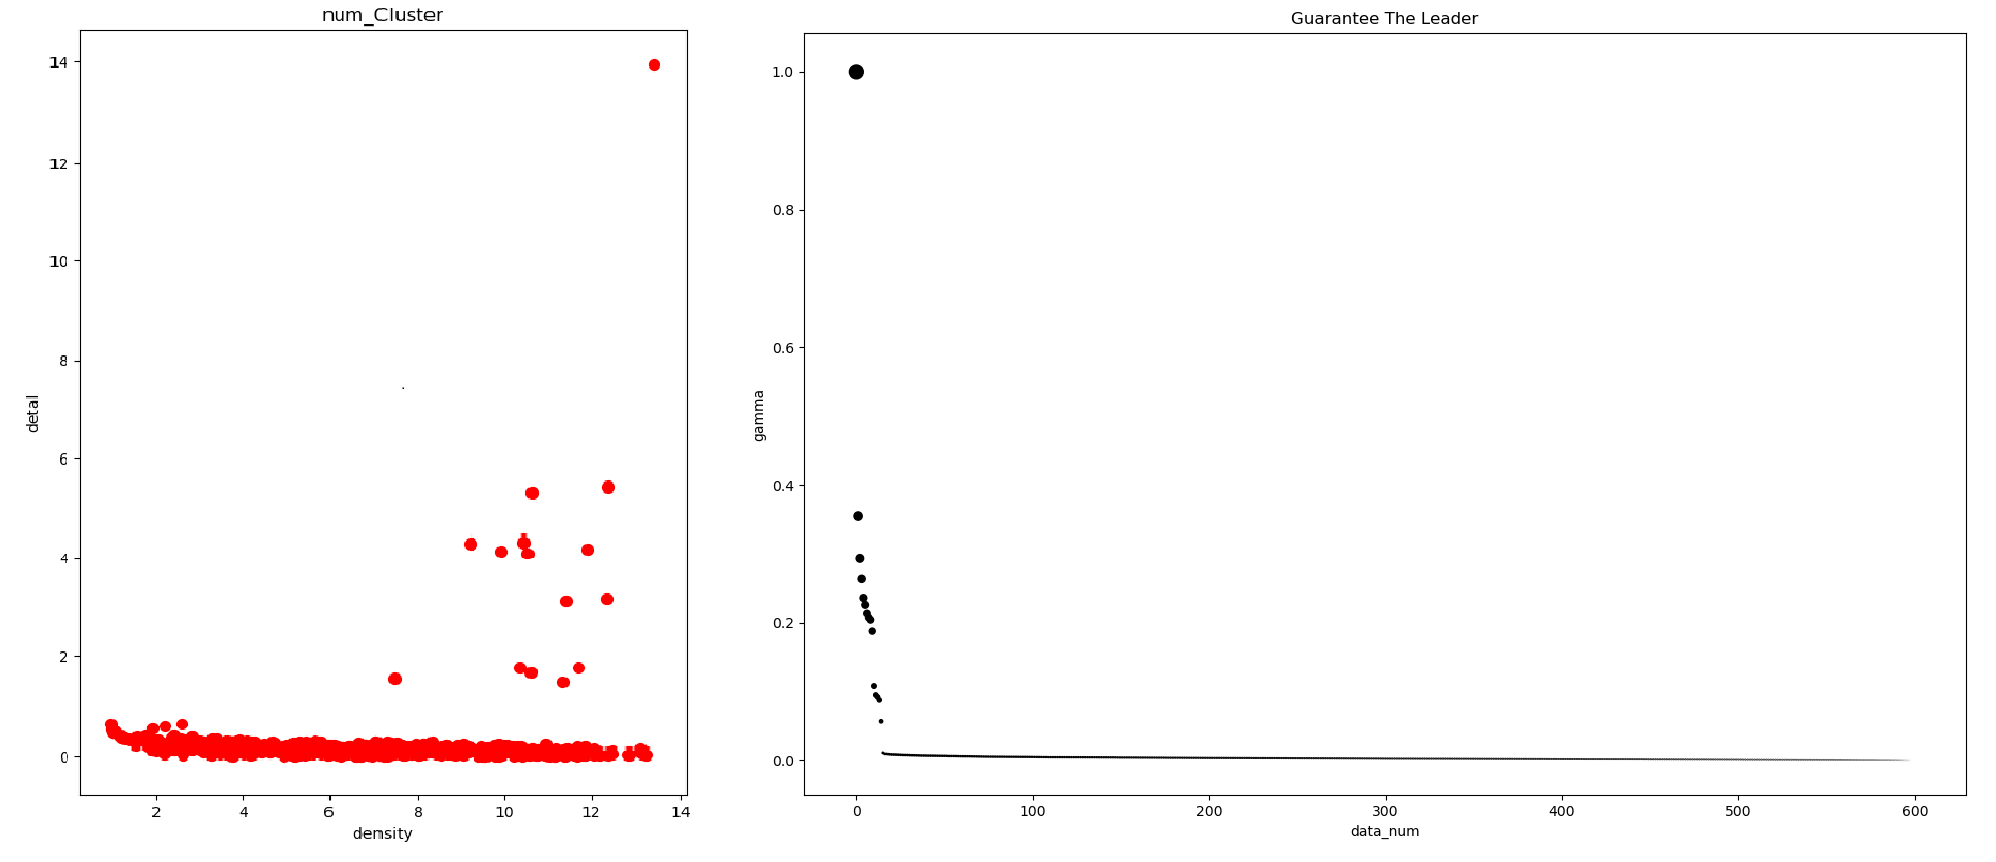
\includegraphics[scale=0.38]{figure/Figure_1.png}%[size][path]
\caption{左图:$\delta$-$\rho$图,横轴为$\rho$,纵轴为$\delta$。\ 右图:$\gamma$图,记录每个点的$\gamma$值}
\label{Figure_1}
\end{figure}

\section{算法原理和步骤}
算法原理可参考上述的算法可行性。下面我们会详细的讲解算法内容。
\subsection{获取距离矩阵}
由论文可知,我们需要的数据基础是所有的点和点之间的距离,所以我们的第一步便是要求出距离矩阵。我在重现论文实验时采用python语言。下面的代码块的功能即是求取距离矩阵。
\begin{lstlisting}[language=python]

def calculate_Distance(data):
    distance_Matrix = np.zeros(shape=(len(data), len(data)))
    for i in range(len(data)):
        for j in range(len(data)):
            if i > j:
                distance_Matrix[i][j] = distance_Matrix[j][i]
            elif i < j:
                distance_Matrix[i][j] = np.sqrt(np.sum(np.power(data[i] - data[j], 2)))
    return distance_Matrix
\end{lstlisting}



\subsection{计算截断距离$dc$}

在获取距离矩阵后,我们需要进行两个最重要的数据的计算:局部密度$\rho$和最小距离$\delta$。由2.1中局部密度$\rho$的定义可以看出,局部密度的计算需要依靠$dc$(截断距离)。所以我们下一步就是获取$dc$。我采用的算法如下:

$dc$为所有点对$(i,j)$距离的前$t\%$。$t$为阈值,可以根据情况自由选择,论文中提到$dc$的取值具有鲁棒性,所以$t$的鲁棒性也是比较好的。$dc$之所以鲁棒性较好,是因为$dc$越大,$\rho$越大,计算$\delta$和选中心点时只比较相对大小,与具体的数值无关。

代码如下:

\begin{lstlisting}[language=python]
def dc_Get(distance_Matrix, tolerance):
    temp_Distance = [] #用于存储所有点对的距离
    for i in range(len(distance_Matrix[0])):
        for j in range(i + 1, len(distance_Matrix[0])):
            temp_Distance.append(distance_Matrix[i][j])
    temp_Distance.sort() #对距离进行升序排序
    dc = temp_Distance[int(len(temp_Distance) * tolerance / 100)] #获取第tolerance%的点对距离作为截断距离
    return dc
\end{lstlisting}


\subsection{获取局部密度$\rho$}
根据上文2.1中可知,我们为局部密度$\rho$提供了两个定义,由于第二个定义(Gaussian kernel)的计算方式涉及到了全体数据,所以我觉得这种方法更加准确些。我写的下列代码提供了两种方法,我把第一个定义的方法给注释了,采用第二种方法。

\begin{lstlisting}[language=python]
def density_Get(distance_Matrix, dc):
    #methon_1
    # density = np.zeros(shape=len(distance_Matrix))
    # for i in range(len(distance_Matrix[0])):
    #     for j in range(len(distance_Matrix[0])):
    #         if distance_Matrix[i][j] <= dc:
    #             density[i] += 1
    # return density
    #methon_2
    density = np.zeros(shape=len(distance_Matrix))
    for index, node in enumerate(distance_Matrix):
        density[index] = np.sum(np.exp(-(node / dc) ** 2))
    return density
\end{lstlisting}


\subsection{获取最小距离$\delta$}
获取最小距离的核心思想,在前面的2.2节中已经介绍。虽然论文中没有提及,但是在代码实现时,我们还需要另外一个量:closest\_Distance,他用于存储比当前点密度高的点集中最近的距离点的索引。我们可以先记住这个量,因为在下面为每个点找归属时会用得到。


\begin{lstlisting}[language=python]
def detal_Get(density, distance_Matrix):
    detal_ls = np.zeros(shape=len(distance_Matrix))#detal_ls存储每个点的detal值
    closest_Distance = np.zeros(shape=len(distance_Matrix), dtype=np.int32)#closest_Distance存储比当前点密度高的点集中最近的距离点的索引
    for index, node in enumerate(distance_Matrix):
        density_Larger_Than_Node = np.squeeze(np.argwhere(density > density[index]))#存储比当前点密度大的点
        if density_Larger_Than_Node.size != 0:#如果有密度大于自己的点
            #所有密度大于自己的点与自己的距离集合(一维数组或者一个数)
            distance_Between_Larger_Node = distance_Matrix[index][density_Larger_Than_Node]
            detal_ls[index] = np.min(distance_Between_Larger_Node)
            min_Distance_Index = np.squeeze(np.argwhere(distance_Between_Larger_Node == detal_ls[index]))
            #存在多个密度大于自己且距离自己最近的点时,选择一个点
            if min_Distance_Index.size >= 2:
                min_Distance_Index = np.random.choice(a=min_Distance_Index)
            if distance_Between_Larger_Node.size > 1:
                closest_Distance[index] = density_Larger_Than_Node[min_Distance_Index]
            else:
                closest_Distance[index] = density_Larger_Than_Node
        #对于最大密度的点
        else:
            detal_ls[index] = np.max(distance_Matrix)
            closest_Distance[index] = index
    return detal_ls, closest_Distance
\end{lstlisting}

\subsection{$\delta$-$\rho$图及$\gamma$(决策)图}
截止到现在为止,我们需要的数据都已经准备好了。前面提到,我们将会根据$\delta\times\rho$来选择聚类的蔟数。在代码实现中,我们首先画出$\delta$-$\rho$图。然后将$\delta$和$\rho$进行标准化后相乘,再画出$\gamma$(决策)图。

在画$\delta$-$\rho$图的过程中,我们顺便画出了原数据散点图,效果见图\ref{figure1_1}。代码如下:
\begin{lstlisting}[language=python]
def show_DensityDetal_And_Dataset(density, detal_Ls, data):
    plt.figure(num=1, figsize=(15, 9))
    #第一个子图为detal-density散点图
    ax1 = plt.subplot(121)
    for i in range(len(data)):
        plt.scatter(x=density[i], y=detal_Ls[i], c='r', marker='o', s=50)
    plt.xlabel('density')
    plt.ylabel('detal')
    plt.title('num_Cluster')
    plt.sca(ax1)
    #第二个子图为原始数据点的散点图
    ax2 = plt.subplot(122)
    for j in range(len(data)):
        plt.scatter(x=data[j, 0], y=data[j, 1], marker='o', c='b', s=50)
    plt.xlabel('axis_x')
    plt.ylabel('axis_y')
    plt.title('set_Data')
    plt.sca(ax2)
    plt.show()
\end{lstlisting}


\begin{figure}[ht]
\centering
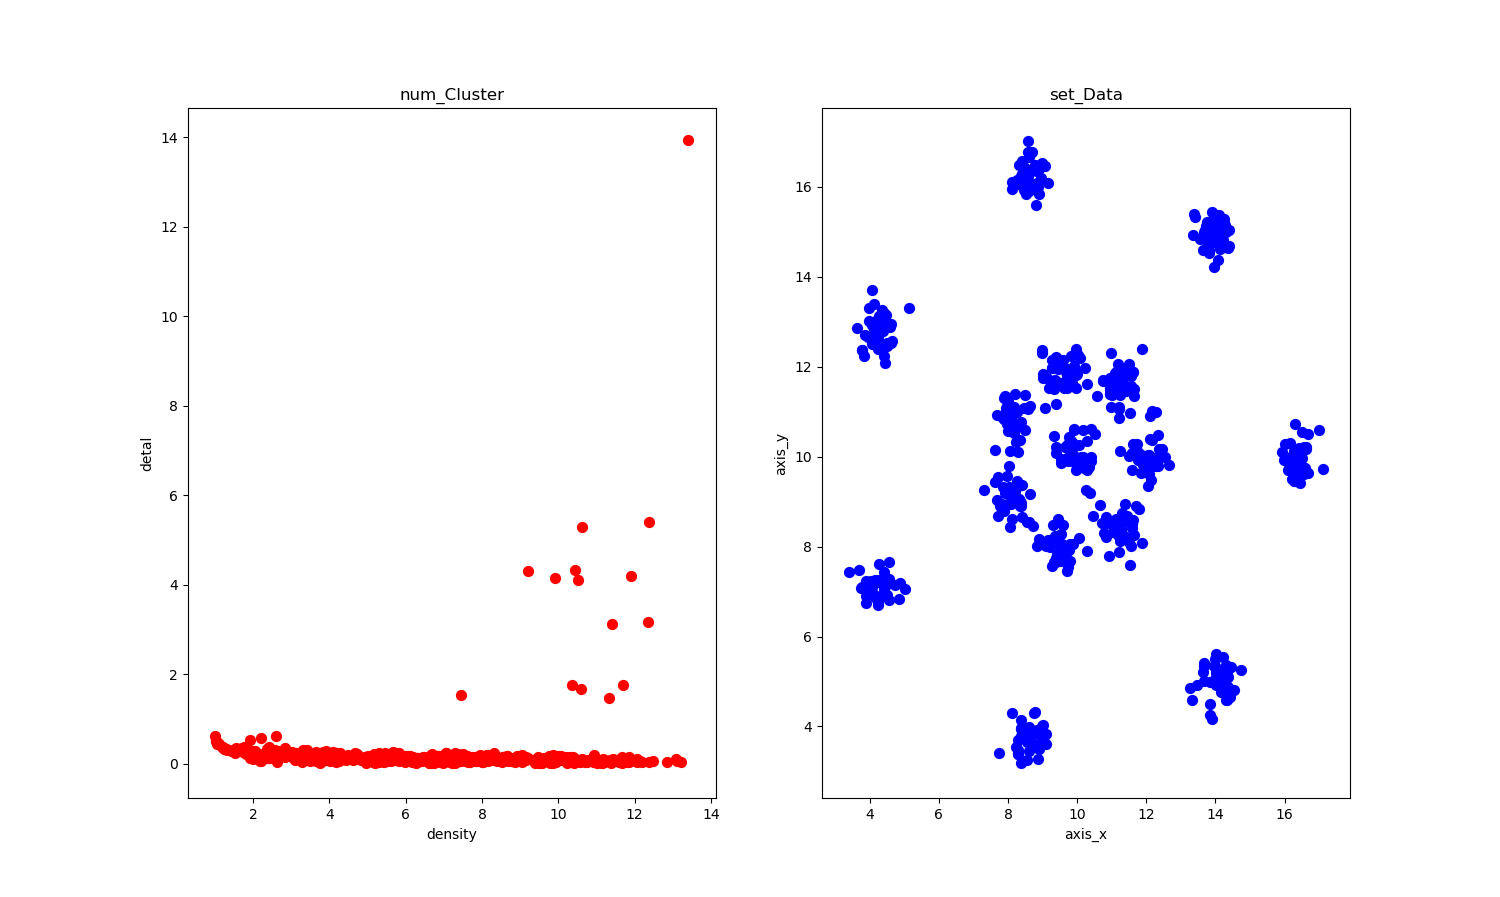
\includegraphics[scale=0.45]{figure/1_1.png}%[size][path]
\caption{左图:$\delta$-$\rho$图,横轴为$\rho$,纵轴为$\delta$。\ 右图:原数据散点图}
\label{figure1_1}
\end{figure}

由图\ref{figure1_1}右图可以看出,该数据集有十五个蔟。由左图可以看出,在左图的右上方也是有十五个点。接着我们用$\gamma$(决策)图来验证一下。


\begin{figure}[ht]
\centering
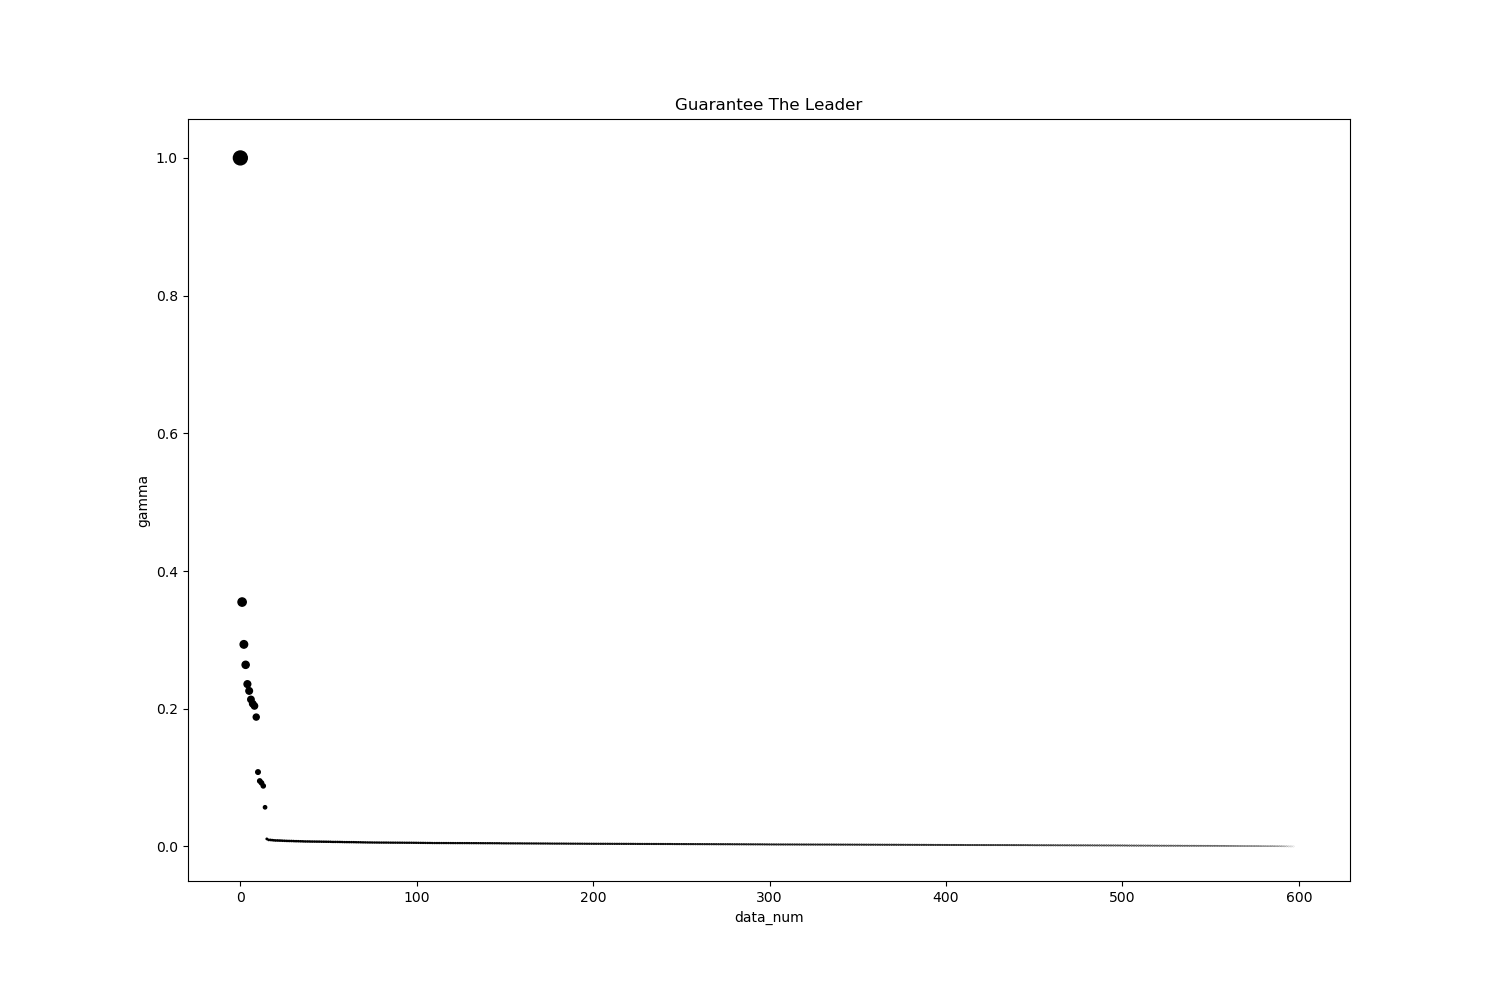
\includegraphics[scale=0.45]{figure/1_2.png}%[size][path]
\caption{$\gamma$(决策)图}
\label{figure1_2}
\end{figure}

$\gamma$(决策)图代码如下:
\begin{lstlisting}[language=python]
def show_Decision_Graph(density, detal_Ls):
    #  由于密度和最短距离两个属性的数量级可能不一样,分别对两者做归一化使结果更平滑
    normal_Density = (density - np.min(density)) / (np.max(density) - np.min(density))
    normal_Detal = (detal_Ls - np.min(detal_Ls)) / (np.max(detal_Ls) - np.min(detal_Ls))
    gamma = normal_Density * normal_Detal
    plt.figure(num=2, figsize=(15, 10))
    plt.scatter(x=range(len(detal_Ls)), y=-np.sort(-gamma), c='k', marker='o', s=-np.sort(-gamma) * 100)
    plt.xlabel('data_num')
    plt.ylabel('gamma')
    plt.title('Guarantee The Leader')
    plt.show()
    return gamma
\end{lstlisting}



由图\ref{figure1_2}也可得出,该数据集的蔟数为15。正如预期的那样,只有具有高局部密度和相对较高的距离的点才是类簇中心。

\subsection{为每个点找到归属}
截止到现在,我们已经找到了类簇中心。那么剩余的点属于哪个蔟呢?这部分论文中并没有介绍,经过查阅相关资料、结合自己的想法,我通过下述算法为每个点找到归属。

前面我们介绍到一个数据量:closest\_Distance,他用于存储比当前点密度高的点集中最近的距离点的索引。我们把所有数据集看成一个森林,每一个蔟看成森林的一棵树。那么可以认为,比当前点密度高的点集中最近的距离点的索引就是其父节点。显然每个蔟的聚类中心就是该树的根节点。并且每个点只有一个父节点。那么根据叶节点依次向上回溯,就可以找到其聚类中心,也即是他的归属蔟。我们前面计算得到的closest\_Distance存储的即是我们刚刚说的“父节点”。

代码如下:
\begin{lstlisting}[language=python]
def clustering(clusters_Num, cluster_Centre_Ls):
    for i in range(len(clusters_Num)):
            while clusters_Num[i] not in cluster_Centre_Ls:
                j = clusters_Num[i]
                clusters_Num[i] = clusters_Num[j]
    cluster_Belong = clusters_Num[:]
    return cluster_Belong  #归属
\end{lstlisting}
\subsection{结果展示}
那么截止到现在,每个点都已找到自己所在的蔟。我们看一下效果,见图\ref{figure1_3}(该部分代码就不再展示,详情见附录)。


\begin{figure}[ht]
\centering
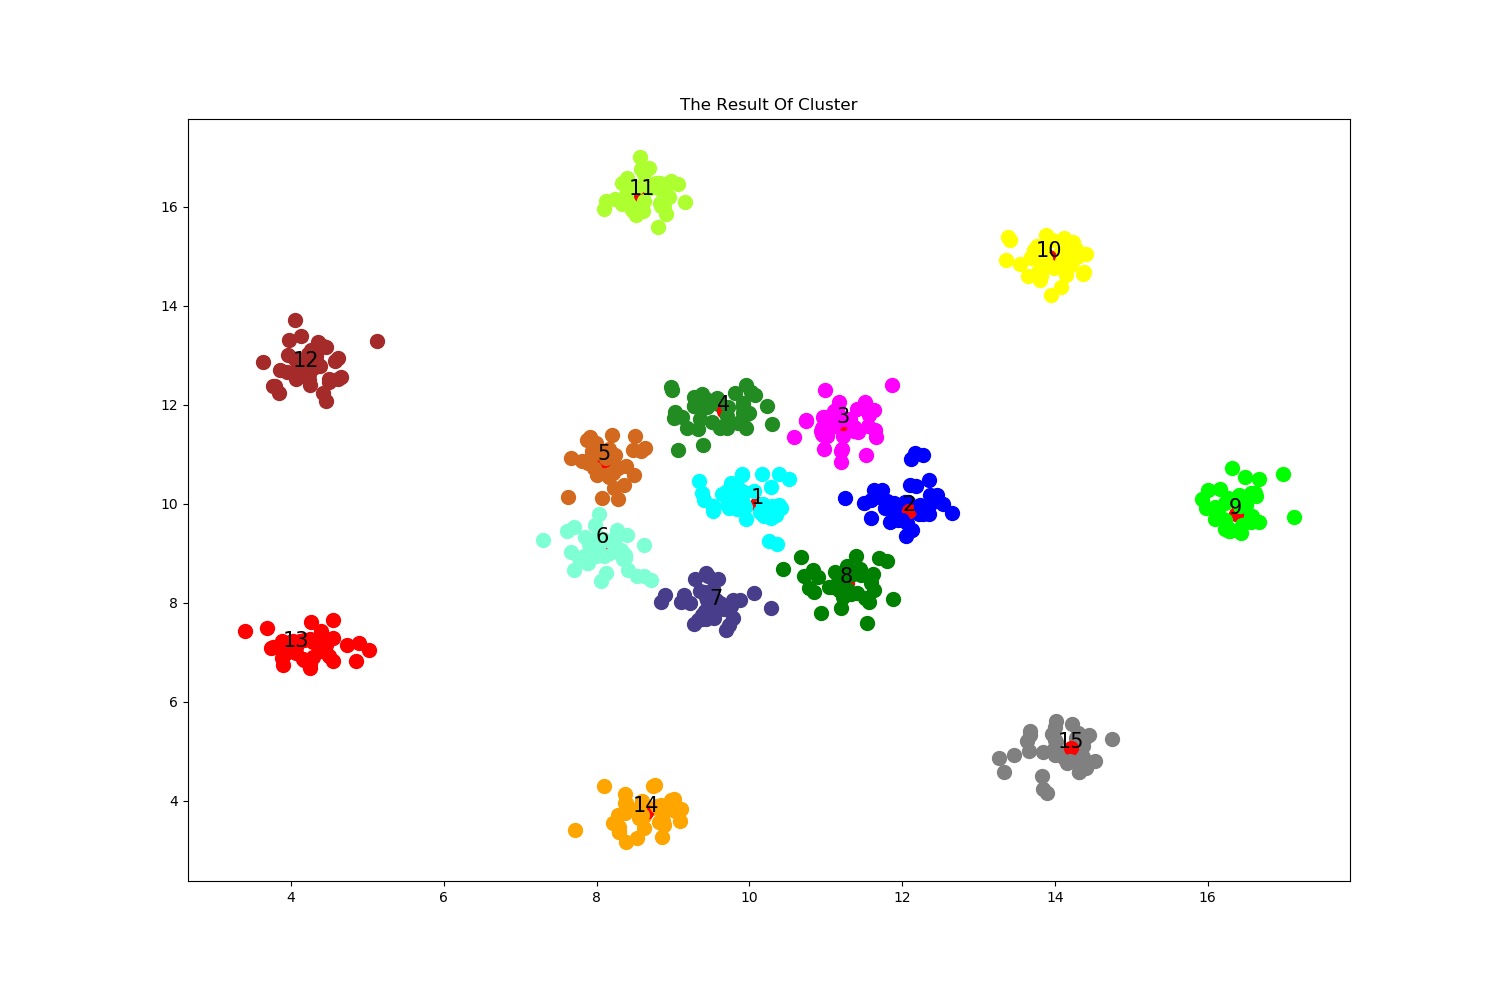
\includegraphics[scale=0.45]{figure/1_3.png}%[size][path]
\caption{结果}
\label{figure1_3}
\end{figure}

\subsection{其他数据集结果展示}
为了说明算法的鲁棒性,我挑选了一些其他类型的数据集进行聚类分析。结果见图\ref{figure2}。由图可以看出应用本算法,这些数据集都能得到不错的效果。

\begin{figure}[ht]
\centering
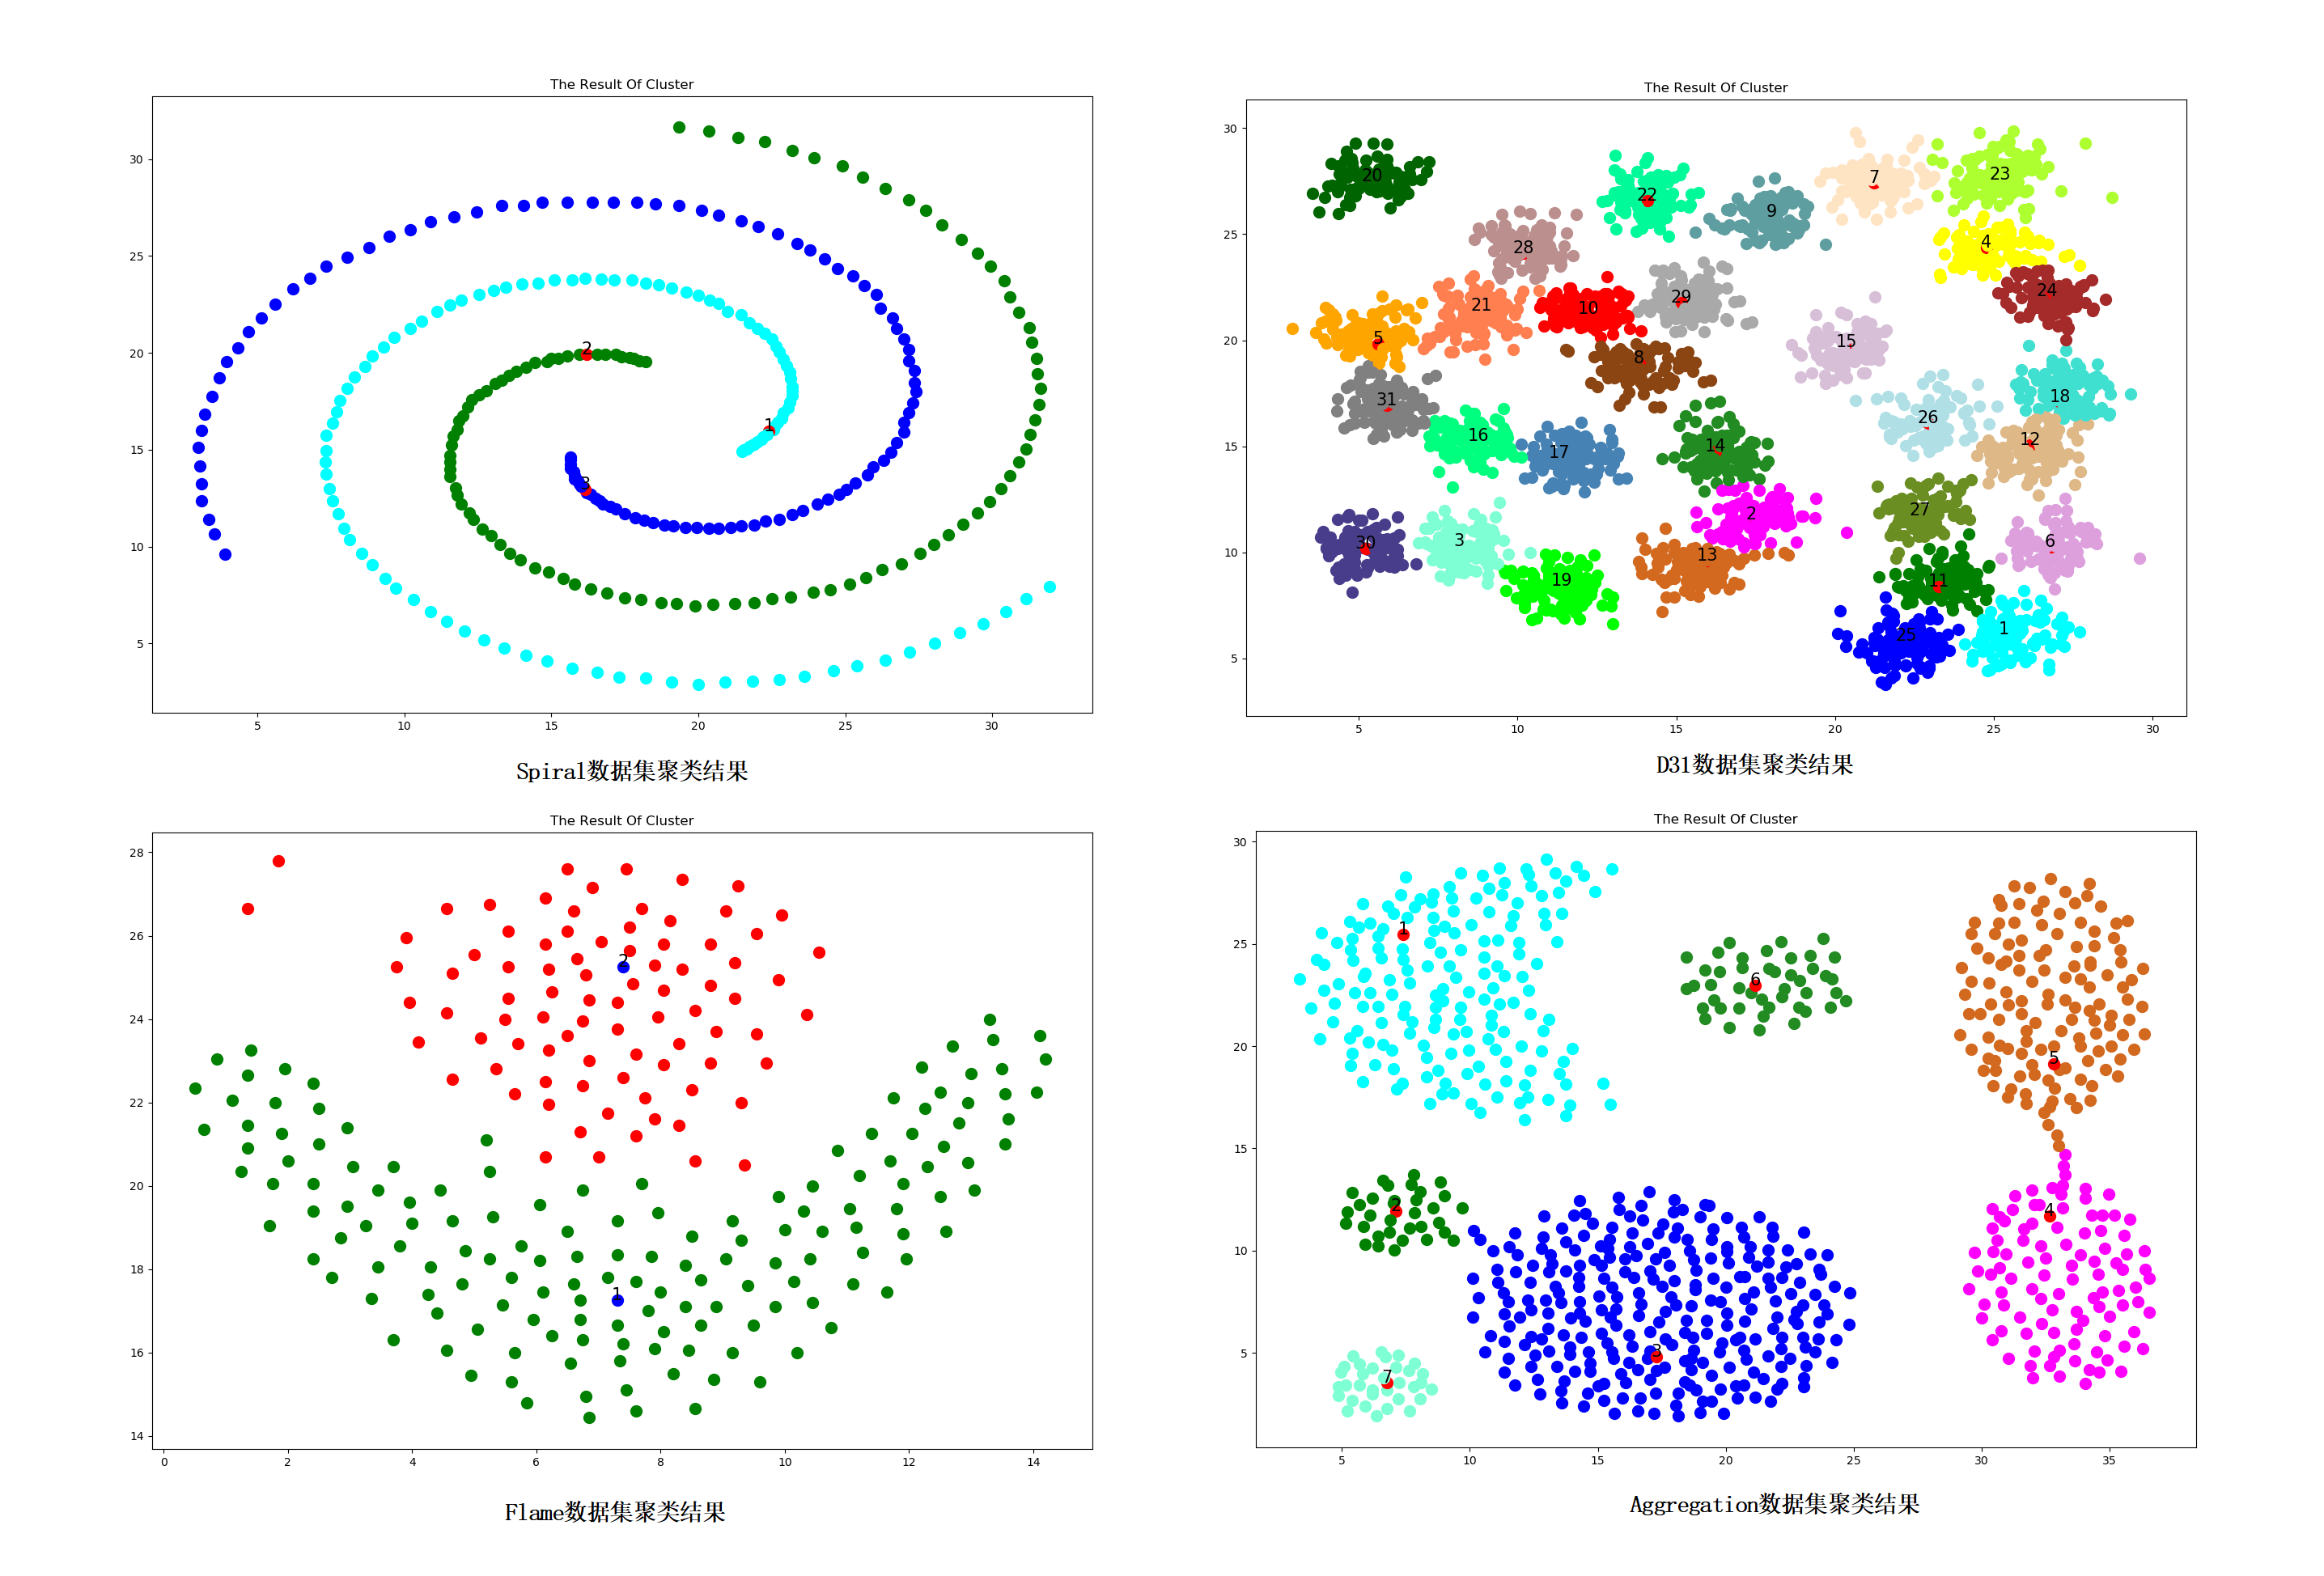
\includegraphics[scale=0.27]{figure/test_2.png}%[size][path]
\caption{}
\label{figure2}
\end{figure}


\section{算法优缺点分析}
\paragraph{算法优点:\\ }


\ \ \  1. 该聚类算法可以得到非球形的聚类结果,可以很好地描述数据分布。

2. 算法复杂度上要比一般的K-means算法的复杂度低,并且不需要迭代。

3. 此算法的只考虑点与点之间的距离,因此不需要将点映射到一个向量空间中。\\

\paragraph{算法缺点:\\ } 


\ \ \  1. 需要事先计算好所有点与点之间的距离。如果样本太大则整个距离矩阵的内存开销特别大,因此如果只需要得到最终聚类中心,则可以考虑牺牲速度的方式计算每一个样本点的和,避免直接加载距离矩阵。

2. 当密度分布不均匀时,效果不好(如Jain数据集)见图\ref{figure2_5},在计算局部密度时并没有考虑局部结构。

3. 应该也不算是缺点吧,毕竟其他方法也没有实现:聚类中心的个数,并不是全自动确定的!!!也是需要人为的对决策图进行判断。
\begin{figure}[ht]
\centering
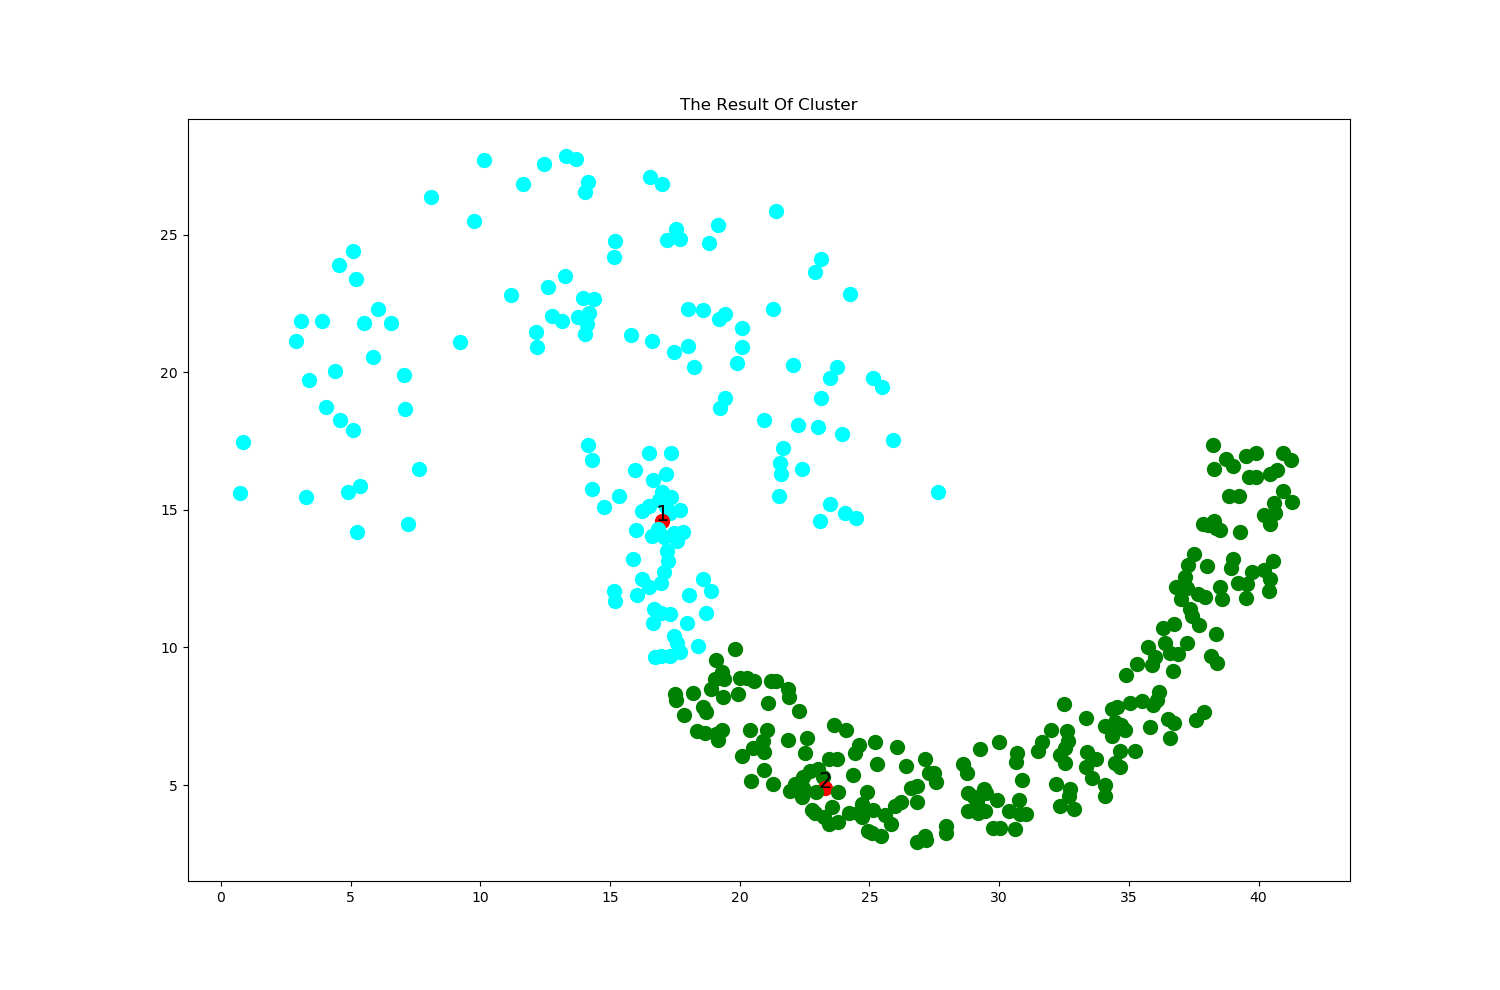
\includegraphics[scale=0.45]{figure/2_5.png}%[size][path]
\caption{Jain数据集聚类结果}
\label{figure2_5}
\end{figure}

\section{总结}

该算法相较于K-means、 K-medoids、DBSCAN等经典算法效果比较好,但是仍然具备一些缺点。比如在图\ref{figure2}右下图Aggregation数据集聚类结果中,如果截断距离$dc$没选择好的话,很有可能会出现右边的两个蔟被聚类成一个蔟的现象(虽然论文说dc的鲁棒性较好),那么这时候聚类的结果可能不如K-means方法。所以从应用的角度来讲,并没有说那个算法一定是强于其他算法的,可能他们针对的问题不同,适用范围不同。所以我觉得合适的算法才是最好的算法。





































%
%=============  附录  ======================
\newpage
\appendix
\section{附录一:python完整源代码}
\textcolor[rgb]{0.98,0.00,0.00}{\textbf{Code}}
\begin{lstlisting}[language=python]
import numpy as np
import matplotlib.pyplot as plt
import collections

def calculate_Distance(data):
    distance_Matrix = np.zeros(shape=(len(data), len(data)))
    for i in range(len(data)):
        for j in range(len(data)):
            if i > j:
                distance_Matrix[i][j] = distance_Matrix[j][i]
            elif i < j:
                distance_Matrix[i][j] = np.sqrt(np.sum(np.power(data[i] - data[j], 2)))
    return distance_Matrix


def dc_Get(distance_Matrix, tolerance):
    temp_Distance = [] #用于存储所有点对的距离
    for i in range(len(distance_Matrix[0])):
        for j in range(i + 1, len(distance_Matrix[0])):
            temp_Distance.append(distance_Matrix[i][j])
    temp_Distance.sort() #对距离进行升序排序
    dc = temp_Distance[int(len(temp_Distance) * tolerance / 100)] #获取第tolerance%的点对距离作为截断距离
    return dc


def density_Get(distance_Matrix, dc):
    #methon_1
    # density = np.zeros(shape=len(distance_Matrix))
    # for i in range(len(distance_Matrix[0])):
    #     for j in range(len(distance_Matrix[0])):
    #         if distance_Matrix[i][j] <= dc:
    #             density[i] += 1
    # return density
    #methon_2
    density = np.zeros(shape=len(distance_Matrix))
    for index, node in enumerate(distance_Matrix):
        density[index] = np.sum(np.exp(-(node / dc) ** 2))
    return density

def detal_Get(density, distance_Matrix):
    detal_ls = np.zeros(shape=len(distance_Matrix))#detal_ls存储每个点的detal值
    closest_Distance = np.zeros(shape=len(distance_Matrix), dtype=np.int32)#closest_Distance存储比当前点密度高的点集中最近的距离点的索引
    for index, node in enumerate(distance_Matrix):
        density_Larger_Than_Node = np.squeeze(np.argwhere(density > density[index]))#存储比当前点密度大的点
        if density_Larger_Than_Node.size != 0:#如果有密度大于自己的点
            #所有密度大于自己的点与自己的距离集合(一维数组或者一个数)
            distance_Between_Larger_Node = distance_Matrix[index][density_Larger_Than_Node]
            detal_ls[index] = np.min(distance_Between_Larger_Node)
            min_Distance_Index = np.squeeze(np.argwhere(distance_Between_Larger_Node == detal_ls[index]))
            #存在多个密度大于自己且距离自己最近的点时,选择一个点
            if min_Distance_Index.size >= 2:
                min_Distance_Index = np.random.choice(a=min_Distance_Index)
            if distance_Between_Larger_Node.size > 1:
                closest_Distance[index] = density_Larger_Than_Node[min_Distance_Index]
            else:
                closest_Distance[index] = density_Larger_Than_Node
        #对于最大密度的点
        else:
            detal_ls[index] = np.max(distance_Matrix)
            closest_Distance[index] = index
    return detal_ls, closest_Distance


def show_DensityDetal_And_Dataset(density, detal_Ls, data):
    plt.figure(num=1, figsize=(15, 9))
    #第一个子图为detal-density散点图
    ax1 = plt.subplot(121)
    for i in range(len(data)):
        plt.scatter(x=density[i], y=detal_Ls[i], c='r', marker='o', s=50)
    plt.xlabel('density')
    plt.ylabel('detal')
    plt.title('num_Cluster')
    plt.sca(ax1)
    #第二个子图为原始数据点的散点图
    ax2 = plt.subplot(122)
    for j in range(len(data)):
        plt.scatter(x=data[j, 0], y=data[j, 1], marker='o', c='b', s=50)
    plt.xlabel('axis_x')
    plt.ylabel('axis_y')
    plt.title('set_Data')
    plt.sca(ax2)
    plt.show()


def show_Decision_Graph(density, detal_Ls):
    #  由于密度和最短距离两个属性的数量级可能不一样,分别对两者做归一化使结果更平滑
    normal_Density = (density - np.min(density)) / (np.max(density) - np.min(density))
    normal_Detal = (detal_Ls - np.min(detal_Ls)) / (np.max(detal_Ls) - np.min(detal_Ls))
    gamma = normal_Density * normal_Detal
    plt.figure(num=2, figsize=(15, 10))
    plt.scatter(x=range(len(detal_Ls)), y=-np.sort(-gamma), c='k', marker='o', s=-np.sort(-gamma) * 100)
    plt.xlabel('data_num')
    plt.ylabel('gamma')
    plt.title('Guarantee The Leader')
    plt.show()
    return gamma


def clustering(clusters_Num, cluster_Centre_Ls):
    for i in range(len(clusters_Num)):
            while clusters_Num[i] not in cluster_Centre_Ls:
                j = clusters_Num[i]
                clusters_Num[i] = clusters_Num[j]
    cluster_Belong = clusters_Num[:]
    return cluster_Belong  #归属


def show_Result(cluster_Belong, data, cluster_Centre_Ls):
    colors = [
        'cyan', 'green', 'blue', 'magenta', 'chocolate',
        'forestgreen', 'aquamarine', 'darkslateblue', 'lime', 'yellow',
        'greenyellow', 'brown', 'red','orange','gray',
        'coral', 'plum', 'burlywood', 'bisque', 'cadetblue',
        'saddlebrown','darkgray', 'rosybrown', 'olivedrab', 'powderblue',
        'turquoise', 'thistle', 'springgreen', 'steelblue', 'darkgreen',
        'mediumspringgreen', 'whitesmoke', 'darksalmon','slategray', 'darkseagreen',
        'azure', 'lawngreen', 'deepskyblue', 'honeydew', 'indianred',
        'darkslategray', 'ivory', 'dodgerblue', 'darkorchid', 'forestgreenblack',

    ]

    # 画最终聚类效果图
    leader_Color = {}
    main_Leaders = dict(collections.Counter(cluster_Belong)).keys()
    for index, i in enumerate(main_Leaders):
        leader_Color[i] = index
    plt.figure(num=3, figsize=(15, 10))
    i = 1
    for node, class_ in enumerate(cluster_Belong):
        #  标出每一类的聚类中心点
        if node in cluster_Centre_Ls:
            plt.scatter(x=data[node, 0], y=data[node, 1], marker="o", s=100, c='r')
            plt.text(data[node, 0], data[node, 1], str(i), ha = 'center',fontsize=15,c='K')
            i += 1
        else:
            plt.scatter(x=data[node, 0], y=data[node, 1], c=colors[leader_Color[class_]], marker='o', s=100)
    plt.title('The Result Of Cluster')
    plt.show()


def main(data):
    distance_Matrix = calculate_Distance(data) #获取距离矩阵,distance[i][j]表示第i个元素和第j个元素之间的欧式距离
    tolerance = 2 #tolerance%用于寻找截断距离,我们本代码中设为2,据论文介绍,截断距离的对聚类的影响不太大
    dc = dc_Get(distance_Matrix, tolerance) #dc为截断距离,本行进行获取dc
    density = density_Get(distance_Matrix, dc) #按照论文公式(1)进行计算每个点的local density
    detal_Ls, closest_Distance = detal_Get(density, distance_Matrix) #detal_ls存储每个点的detal值,closest_distance存储比当前点密度高的点集中最近的距离点的索引
    show_DensityDetal_And_Dataset(density, detal_Ls, data) #展示density-detal散点图和原始data图
    density_Multiply_Detal_Sort = show_Decision_Graph(density, detal_Ls) #展示决策图,返回标准化后的density和detal乘积(已经进行排序)
    clusters_Num = int(input('input clusters num:')) #根据决策图输入聚类数
    cluster_Centre_Ls = np.argsort(-density_Multiply_Detal_Sort)[: clusters_Num] #获取聚类中心点的集合
    cluster_Belong = clustering(closest_Distance, cluster_Centre_Ls)  # 确定各点的最终归属(哪个司令)
    show_Result(cluster_Belong, data, cluster_Centre_Ls)  # 展示结果


if __name__ == '__main__':
    pathname = r'data\Jain.txt'
    data = np.loadtxt(pathname, delimiter='	', usecols=[0, 1])
    main(data)
\end{lstlisting}






\section{附录二:GitHub链接}
在链接中包含了论文的pdf文件、算法实现的代码、数据集、论文笔记和LaTeX模板。
\begin{enumerate}
\item \textcolor{blue}{ \href{https://github.com/Venture-Zhao/Clustering-by-fast-search-and-find-of-density-peaks-Paper-notes}{点击跳转}}
\end{enumerate}



\end{document}
%%%%%%%%%% 结束 %%%%%%%%%%